\documentclass[12pt]{article}

%%% Packages %%%

\usepackage[utf8]{inputenc}
\usepackage{titlesec}
\usepackage{graphicx}
\usepackage[margin=1in]{geometry}
\usepackage{eurosym}
\usepackage{makecell}

%%% Styles %%%

\titleformat{\chapter}{\normalfont\huge}{\thechapter.}{20pt}{\huge\it}

\titleformat{\paragraph}
{\normalfont\normalsize\bfseries}{\theparagraph}{1em}{}
\titlespacing*{\paragraph}
{0pt}{3.25ex plus 1ex minus .2ex}{1.5ex plus .2ex}

\bibliographystyle{abbrv}

%%% Document information %%%

\title{
	{
	
\includegraphics[width=0.7\linewidth]{images/logo-fib.png}	
	\vspace{1cm}
	\textbf{\\New real-time GNSS algorithms for detection and measurement of potential geoeffective stellar flares}
}
\author{\textbf{Author}\\
	David Moreno Borr\`as
	\\ \\
	\textbf{Supervisor}\\
	 Manuel Hernández-Pajares}
\date{\today}
}


%%%%%%%%%%%%%%%%%%%%%%%%%%%%%%%%%%%
%%%%%%% Start of document %%%%%%%%%
%%%%%%%%%%%%%%%%%%%%%%%%%%%%%%%%%%%

\begin{document}
	
\pagenumbering{arabic}
\clearpage
\maketitle
\thispagestyle{empty}
\clearpage


\tableofcontents
\thispagestyle{empty}
\newpage
\listoftables
\thispagestyle{empty}
\clearpage

%%%%%%%%%%%%%%%%%%%%%%%%%%%%%%
%%%%%%% Introduction %%%%%%%%%
%%%%%%%%%%%%%%%%%%%%%%%%%%%%%%

\section{Introduction}

Solar flares are sudden electromagnetic emissions on the Sun’s surface that release large amounts of magnetic energy. These flares emit radiation that has an effect on Earth’s ionosphere electron content and therefore the many satellites orbiting it. \cite{hernandez2012gnss}\\

Several NASA missions that aim to detect these and other flares from far-away stars exist, like the Swift and Fermi missions, these satellites, however, perform this by using their instruments to study the gamma-ray, x-ray and ultraviolet radiation bands. \cite{gehrels2013gamma}\\

The aforementioned ionosphere electron content variation, however, makes it possible to detect these flares with a more indirect approach: using data from the satellites belonging to global positioning systems.\\

As the sudden increase of electron content in the ionosphere has an effect on the signals these satellites receive and send, this data can be used to detect flares by using the appropriate algorithms. Parameters such as the angle between the Sun and the zenith of the Earth, or the Total Electron Content (TEC) in the air have to be taken into consideration for them to work. \\

This is already feasible with flares that have the Sun as a source, so our goal is to, first of all, expand on that by detecting these flares without knowing the location of the Sun, and then apply that to study if it is possible to detect flares from far-away stars by developing the appropriate algorithms.\\

Therefore, the main objective of our project is to study the feasibility of the detection of stellar flares using Global Navigation Satellite System (GNSS) or Global Positioning System (GPS) measurements without knowing the location of the source. If this is possible, it could be extended to real-time detection.\\

The aim of this document is to give a detailed description of the project, its scope and context.\\

%%%%%%%%%%%%%%%%%%%%%%%%%%%%%%%%%%%%%
%%%%%%% Scope of the project %%%%%%%%
%%%%%%%%%%%%%%%%%%%%%%%%%%%%%%%%%%%%%

\newpage
\section{Scope of the project}

Now that we have defined the problem that we want to solve, we proceed to define the scope of our project: how are we going to tackle it, and what could be some obstacles that might arise during its development.

\subsection{Objectives}

For a possible progression we could present the objectives of the project as follows:

\begin{itemize}
  \item To understand how the already existing algorithms for solar flare detection work, and see how we can apply them to the challenging scenario of far-away stars.
  \item Be able to work with GNSS data in order to use it as the input for our algorithms and compare that to flares registered by satellites like Swift or Fermi.
  \item Using this data, developing new algorithms that can perform the detection using solar flares first but without knowing the origin of the source, that is, not only detecting the solar flare, but the position of the Sun relative to the Earth.
  \item Applying this to the challenging scenario of far-away stars without knowing the position of the potential ionizing source.
  \item Prepare these algorithms to be applied for real-time data.
\end{itemize}

\subsection{Scope}

We need to study the impact of stellar flares on the Earth’s ionosphere by adapting the already existing algorithms that work with the Sun, but without knowing the source of the flare to see if we can apply this method to the scenario of far-away stars.\\

And finally, if possible, using the result to adapt the solution to run in real-time.

\subsection{Methodology and rigor}

The project has been planned to assure that it is developed in a bottom-up style, from less to most challenging objectives because every step of the development relies on the previous one to work. Therefore, as we have specified before, the project is going to start by working with a less-challenging scenario: the Sun.\\

The objective is to develop an algorithm that is able to detect solar flares without knowing their location, so we can later extend it to far-away stars. Before starting with this algorithm, a first approach will be done knowing the location of the source (the location of the Sun relative to the Earth in the moment of a recorded flare) so we can assure that the computations are correct.

Parallel to this, the feasibility of detecting far-away flares will be studied, using the currently existing algorithms \cite{hernandez2012gnss} but applied to recorded stellar flares, rather than Solar. If it is possible, we will adapt the previously developed algorithm so that it works not only with the Sun, but far-away stars (of which we don't know the location).\\

Finally, if any of the two objectives is successful, the algorithms will be adapted to run in real time: instead of just testing them with previous data and checked against recorded events, they will be run in real time using the latest available GNSS data.

\paragraph{Development tools}

Git and GitHub are going to be the tools used for version control and code maintenance.\\

The platform we will be developing on will be Linux, and regarding programming languages, C-Shell will be used for scripts, AWK for the pre-processing of data and Fortran for the main algorithms. \\

Fortran was used for computing the relation between the Sun’s angle with the Earth’s zenith and the VTEC given by the data of a satellite, but a new part of our algorithm that didn’t have to be considered with the previous ones is how to traverse the set of GNSS satellites of the whole globe and decide which ones should compute this relation, that is, efficiently consider which satellites could possibly lead us to results, instead of checking that for all of them with a brute force algorithm.

We will consider if there’s any alternative that may bring us more benefits than using Fortran for this part. \\

Others tools might be used in the process, for example we could use something like Python to scrap the website of the Swift satellite for the data we want or download it and process it with C-shell or Bash.\\

Regarding the GNSS data we are going to be using, this is made available by the  International GNSS Service (IGS). This voluntary federation offers open access GNSS data that can be used to obtain ionospheric information. \cite{hernandez2009igs}

\paragraph{Progress monitoring}

In order to track the progress and comment on the results, a weekly meeting with the project director is organized, where we set several “Action Items” to be done during the week prior to our next meeting. Additionally, communication via email is also a possibility for any problems that might arise during the week.

\paragraph{Validation of the results}

Data from the Swift or Fermi missions is going to be used for the validation of our results. Using past GNSS data, we will develop algorithms that use it to detect flares and the location of the source. 

Swift and Fermi data will have information about the flares, so we will compare our results to see if we really detected a flare. This will also be done for the scenario of far-away stars.

Regarding the last phase, the algorithms running in real time, the only way to validate the results is to wait for any matching data from the Swift and Fermi databases.

\subsection{Obstacles and risks of the project}

Although we have stated the objectives that we aim to follow in our project, its development may be hampered by some common problems that appear when developing software and algorithms, and others that may arise due to the nature of our problem.

\paragraph{Understanding of the problem}

The problem has a considerable physics background that I, as a Computer Science student, lack the knowledge to completely understand it. Although a basic knowledge in the field will suffice for developing the algorithms, not having a background in physics might lead to confusion at some point.

\paragraph{Unfeasibility of the solution}

The problem that we want to solve is clear: detecting stellar flares from far-away stars. This has been studied for some cases \cite{martinez2016first}, concluding that we face the possibility that the proposed solution is not totally feasible due to the nature of the problem: flares from far-away stars will not have an impact on the ionosphere as noticeable as the one from the sun, so it may be difficult, or even impossible, for them to be detected in some cases.

\paragraph{Interferences with the Sun}

With the Sun, only the daylight hemisphere is studied for the detection of flares using GPS data (it is the only one flares' effects can reach)

In our case we don’t have a fixed source, but rather aim to find it. Flares could be having an effect on any part of the ionosphere so it may not be possible to study their effect on the daylight hemisphere because of the Sun’s (presumably) higher effect on it. 

Because of this factor we might have to focus only on the night hemisphere and we would be missing on possible flares.

\paragraph{Understanding previous algorithms}

It is often difficult to understand code that has not been written by oneself, let alone understanding complex algorithms without any previous knowledge. This could be another possible obstacle, as the study of the previously developed algorithms will play an important role in the development of ours.

\paragraph{Bugs}

As we will be writing code it is clearly possible that we face problems with bugs that may appear in the process.

\paragraph{Computational power}

Taking into consideration we may be dealing with large volumes of data, its processing may be another challenge for the project, we will have to find efficient ways to do so and think about which strategies will work best in our algorithms.

%%%%%%%%%%%%%%%%%%%%%%%%%%%%%%%%
%%%%%%% Contextualization %%%%%%
%%%%%%%%%%%%%%%%%%%%%%%%%%%%%%%%
\newpage
\section{Contextualization}

In this section we aim to give a brief description of the area of interest of the project and present which actors are going to be involved in its development.

\subsection{Areas of interest}

The problem has a clear background in the field of \textbf{physics} and \textbf{astronomy}. I wanted to work on a project related to astronomy to see how computer science could be applied to this field. 

Although there’s an important theory part behind, the weight of the project lies in developing the \textbf{algorithms}.\\

On the other hand, the \textbf{study of large sets of data} is another area of interest of the project, and how we can use all the GNSS data efficiently in order to generate new information.\\

If successful, it could also be expanded with other interesting fields like AI or Machine Learning to aid in the detection or classification of these flares, for example.

\subsection{Stakeholders}

\paragraph{Developers}

The project is being developed by myself, David Moreno Borràs. Computer Science student at the Barcelona School Of Informatics (FIB).\\

I will be writing the documentation and working on the project but as I lack the knowledge of the more theoretical part of the project, the director, Manuel Hernández-Pajares, will aid me with these aspects, as this is his area of expertise.

\paragraph{Directors}

The director of the project is Manuel Hernández-Pajares, professor from the department of Applied Mathematics at the Technical University of Catalonia (UPC). 

He has conducted several studies related to the field of this project (ionospheric sounding and GNSS navigation) and is the creator of the already existing algorithms used for detecting solar flares, so he can assist me when understanding how they work and how they can be used to develop the new ones.

\paragraph{Benefited Actors}

The mainly benefited actors would be astronomers because this technique would allow to use GPS as an astronomical instrument for the measurement of the Sun’s EUV radiaton.\\

This would be a ground system with zero cost to detect stellar flares by using free, publicly available GNSS data.

\subsection{State of the art}

In this section we will discuss the situation of the project regarding previous studies on the field, and what does it aim to extend upon.          

\paragraph{Far-away stars}

Detection of flares by far-away stars and Gamma-Ray Bursts, powerful explosions caused by supernovas (the result of a dying star) are studied by the Swift or Fermi missions \cite{gehrels2013gamma}, for example. As will be seen later in the sustainability section, our project, if successful, would be presenting an alternative to these telescopes with less complex technology.

A first-study of this topic was done in the Master Thesis \textit{“First study on the feasibility of Stellar Flares detection with GPS”} \cite{martinez2016first} written by David Martinez Cid and also directed by Manuel Hernández-Pajares.

The project concluded by stating that more stellar flares should be studied in order to determine whether the solar flare detection algorithms are able to detect stellar flares, which is what we intend to do with new algorithms that don’t rely on the location of the source.

It is a challenging scenario due to the location of the source, as it will not have the same impact on Earth as flares from the Sun, but considering more powerful stars exist, their effects might be able to reach Earth.

\paragraph{Solar Flares}

As mentioned before, the project director, Manuel Hernández-Pajares has conducted several studies on this topic and presented different solutions as can be seen in \textit{“GNSS measurement of EUV photons flux rate during strong and mid solar flares”} \cite{hernandez2012gnss} where a detailed explanation of the case is presented and \textit{“GPS as a solar observational instrument: Real-time estimation of EUV photons flux rate during strong, medium, and weak solar flares”} \cite{singh2015gps}, in collaboration with the Indian Institute of Technology.\\

In both of these papers the use of GPS measurements is presented as an accurate Solar observational tool using the GNSS solar flare activity indicator (GSFLAI) algorithm.\\

The project would be expanding on this topic by presenting a solution that does not consider the source of the flare, that is, detecting it without knowing the position of the Sun relative to the Earth. This would be a tool able to determine the position of the Sun and the event of a solar flare without a dedicated satellite, using only free, open-source data.

%%%%%%%%%%%%%%%%%%%%%%%%%%%%%%
%%%%%%% Planning and scheduling %%%%%%%%%
%%%%%%%%%%%%%%%%%%%%%%%%%%%%%%
\newpage
\section{Planning and scheduling}

The aim of this document is to present the tasks and stages of the project and how are they going to be planned and scheduled so the project meets its objectives within the given deadlines.

Because we rely on some stages of the project to work before we begin to tackle others, this planning might be updated as the project progresses, perhaps because a part took longer to develop than expected or (luckily) less.

%%%%%%%%%%%%%%%%%%%%%%%%%%%%%%%%%%%%%
%%%%%%% Task description %%%%%%%%
%%%%%%%%%%%%%%%%%%%%%%%%%%%%%%%%%%%%%
\subsection{Task description}

In this section a description of each task is presented in a similar order to that which will be seen later in the planning section.

\paragraph{1 Introduction to the problem}

Study past research papers related to the problem to gain some background on the project, this includes the following topics:

\begin{itemize}
  \item The use of GNSS data as a solar flare meter. Some research papers about this topic were discussed in the State of the Art section, most of them written by the director, Manuel Hernández-Pajares. \cite{hernandez2012gnss}
  \item Solar and stellar bursts and their effect on Earth’s ionosphere. The aforementioned papers give a brief introduction to the topic, although others can be found that cover the topic with more depth. \cite{mitra1974ionospheric}
\end{itemize}

\paragraph{2 GEP}

The GEP course is done early in the project to help with the documentation of the thesis, understanding the scope and context of the project, and its planning. Its different stages are:

\begin{itemize}
	\item Context and Scope of the project
	\item Project planning
	\item Budget and sustainability
\end{itemize}

This also involves a final deliverable that includes the previously listed parts but taking into consideration the feedback of the professors of the course.

Finally, an oral presentation will be done describing the work done during this course, which will also be a starting point of the final presentation of the thesis.

\paragraph{3 Feasibility of the detection of flares from far-away stars}

Before developing the algorithms to be able to perform this without knowing the source of the flare, a study should be done with the already existing algorithms. This is one of the most challenging problems of the project as it is not clear yet if this is possible.

To do this, we will use open-source data from missions like Swift or Fermi (satellites that are able to detect flares or burst) and see if there is any correlation between that data and the results given by the algorithms that detect solar flares.

\paragraph{4 Detection of solar flares with no information about the location of the Sun}

This task will be done in parallel to the previous one. The current algorithms are able to, knowing the position of the Sun, study if any flares have had an effect on the ionosphere, detectable by the satellites belonging to GNSS. 

We aim to do the same, but assuming we don’t have any information about the position of the Sun relative to the Earth. This is an important task for the project, because it will be necessary when expanding it to far-away stars, of which we ignore the location.

\paragraph{5 Detection of stellar flares in real-time}

If the previous systems work, instead of studying flares using past GNSS data and checking that the results match detections by satellites like Swift or Fermi, we will use the latest available data to detect them in real-time, without knowing the location of the ionizing source. For this to work the detection of far-away stars using this system and the detection of solar flares without knowing the location of the Sun have to work properly.

\paragraph{6 Writing the report}

This task will be done in parallel to the rest. As we perform the other tasks a memory of the project will be written giving a detailed explanation of all the phases, the methodology and development of the solutions, problems or obstacles that might have appeared, and the final results of each of them. 

\paragraph{7 Final presentation}

The final task, once the report of the project is finished, is to prepare an oral presentation for the defense of the thesis. This will try to cover all the progress of the work done during the last months as concisely as possible, presenting the results, obstacles that may have appeared and solutions presented for the problems.

%%%%%%%%%%%%%%%%%%%%%%%%%%%%%%%%
%%%%%%%%%% Time table %%%%%%%%%%
%%%%%%%%%%%%%%%%%%%%%%%%%%%%%%%%
\subsection{Time table}

Table 1 shows the estimation of the amount of hours that will have to be dedicated for the completion of each task. The expected amount of dedicated hours to the project is 18 ECTS x 30h/ECTS = 540 hours, of which 3x30 = 90 hours are dedicated to the GEP course.

\begin{table}[h!]
	\centering
	\begin{tabular}{||c c||} 
		\hline
		Task & Dedication Time (hours) \\ [0.5ex] 
		\hline\hline
		Introduction & 20  \\ 
		\hline
		GEP & 90  \\
		\hline
		Study of flares from far-away stars & 120 \\
		\hline
		Detection of solar flares & 120  \\
		\hline
		Detection in real-time & 100  \\ 
		\hline
		Writing report & 90  \\ 
		\hline
		Final presentation & 4 \\
		\hline\hline
		Total & 544  \\
		\hline
	\end{tabular}
	\caption{Dedication time to each of the tasks}
	\label{table:1}
\end{table}

Taking into consideration the project will span 14 weeks, a weekly dedication of 34 hours is possible for the project planning to work as scheduled.

%%%%%%%%%%%%%%%%%%%%%%%%%%%%%%%%
%%%%%%%%%% Scheduling %%%%%%%%%%
%%%%%%%%%%%%%%%%%%%%%%%%%%%%%%%%
\subsection{Scheduling: Gantt chart}

Having started mid-February, the development of the project will span between 4 or 5 months as the oral presentations are scheduled for the first week of July. 

The report should be handed in one week prior to the lectures, so for the planning, our objective is to finish the project a week before: Friday, 21th of June, so that there is enough time to revise it and make any convenient changes.

To visually represent the schedule of the planning, a Gantt chart is shown below in Figure 1. This chart has been generated using the online tool teamgantt.com: 

\vspace{0.25cm}

\begin{figure}[ht]
	\centering	
	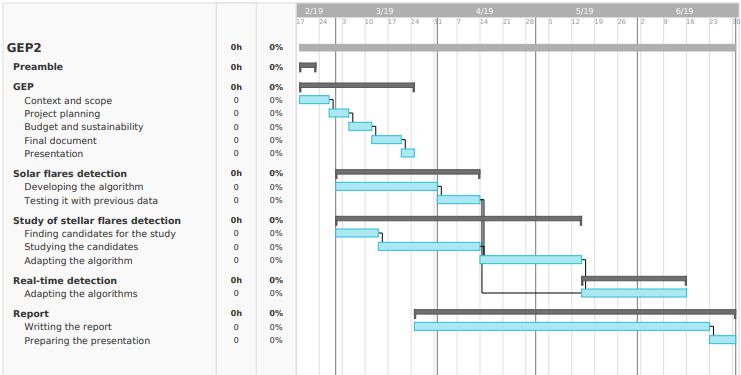
\includegraphics[width=0.9\linewidth]{images/GanttChart.png}
	\caption{Gantt chart with the planning of the project }
\end{figure}
	

%%%%%%%%%%%%%%%%%%%%%%%%%%%%%%%%
%%%%%%%%%% Action plan %%%%%%%%%%
%%%%%%%%%%%%%%%%%%%%%%%%%%%%%%%%

\subsection{Action plan}

Our idea is to work in the presented order as planned in the the previous sections, some tasks depend on previous ones to be finished to continue, and others are going to be done in parallel, like writing the report.

The project was been scheduled as previously presented, but if the dedication for some of the tasks is more than expected, the schedule should be modified as the project progresses to adapt to these situations. Another factor that might have an effect on our scheduling are some problems that might appear during the development of the project, this may cause delays and that will force us to reschedule the project planning, some of which are presented below.

As seen in the methodology section, a weekly meeting with the supervisor is held, so if any delays have appeared during the week, the schedule can be changed accordingly.

\paragraph{Understanding of the problem}

The problem has a considerable physics background that I, as a Computer Science student, lack the knowledge to completely understand it. Although a basic knowledge in the field will suffice for developing the algorithms, not having a background in physics might lead to confusion at some point, and will make it more difficult to understand what does the algorithm have to exactly do.

\paragraph{Understanding previous algorithms}

It is often difficult to understand code that has not been written by oneself, let alone understanding complex algorithms without any previous knowledge. This could be another possible obstacle, as the study of the previously developed algorithms will play an important role in the development of ours.

\paragraph{Bugs}

As we will be writing code it is clearly possible that we face problems with bugs that may appear in the process.

\subsection{Resources}

Several tools that will be studied in detail in the following section, along with the cost they imply, will be needed for the development of the project. These resources can be classified in three major groups:

\paragraph{Software resources}

Many software tools will be needed for the development of the project, although all of them will be free and open-source. All the used tools are listed in the next section, although some of the main ones are Git, which will be used for version control, everything will be running on Linux and \LaTeX\ will be used for the reports. 

\paragraph{Hardware resources}

In this case only a computer will be needed, we will be relying on data that has been obtained using far more complex technologies (all the satellites and hardware involved in GNSS) but a computer and its peripherals will be the only hardware used during the project.

\paragraph{Human resources}

One person will be developing the project and will have three roles: the project manager (time management and writing the report), software developer (developing the necessary algorithms) and tester (testing said algorithms).

%%%%%%%%%%%%%%%%%%%%%%%%%%%%%%
%%%%%%% Cost estimation %%%%%%
%%%%%%%%%%%%%%%%%%%%%%%%%%%%%%

\section{Cost estimation}

In the following sections, an estimation of the cost is presented. These are going to be divided in four major sections: hardware, software, human resources and indirect costs. Because  some of the tasks will use the same resources, they have been grouped, but those that use different resources will be studied in a different section.

\subsection{Software resources}

\paragraph{Common resources}

\begin{table}[h!]
	\centering
	\def\arraystretch{1.2}
	\begin{tabular}{|c c c c c|} 
		\hline
		Product & Units & Price & Useful life (years) & Amortization \\ [0.5ex] 
		\hline\hline
		Ubuntu 18.04 & 1 & 0 \euro & - & 0 \euro \\ 
		\hline
		Google Chrome & 1 & 0 \euro & - & 0 \euro \\
		\hline
		Evince & 1 & 0 \euro & - & 0 \euro \\
		\hline\hline
		Total &  & 0 \euro &  & 0 \euro \\
		\hline
	\end{tabular}
	\caption{Software costs}
\end{table}

\newpage

\paragraph{Developing the algorithms}

\begin{table}[h!]
	\centering
	\def\arraystretch{1.2}
	\begin{tabular}{|c c c c c|} 
		\hline
		Product & Units & Price & Useful life (years) & Amortization \\
		\hline\hline
		Git & 1 & 0 \euro & - & 0 \euro \\ 
		\hline
		GitHub & 1 & 0 \euro & - & 0 \euro \\
		\hline
		Sublime Text 3 & 1 & 0 \euro & - & 0 \euro \\
		\hline
		Python & 1 & 0 \euro & - & 0 \euro \\
		\hline
		GNSS Data & 1 & 0 \euro & - & 0 \euro \\
		\hline
		GFortran & 1 & 0 \euro & - & 0 \euro \\
		\hline\hline
		Total &   & 0 \euro &  & 0 \euro \\
		\hline
	\end{tabular}
	\caption{Software costs}
\end{table}

\paragraph{GEP and writing the report}

\begin{table}[h!]
	\centering
	\def\arraystretch{1.2}
	\begin{tabular}{|c c c c c|} 
		\hline
		Product & Units & Price & Useful life (years) & Amortization \\
		\hline\hline
		LibreOffice & 1 & 0 \euro & - & 0 \euro \\ 
		\hline
		LaTeX & 1 & 0 \euro & - & 0 \euro \\
		\hline
		TeamGantt & 1 & 0 \euro & - & 0 \euro \\
		\hline\hline
		Total &   & 0 \euro &  & 0 \euro \\
		\hline
	\end{tabular}
	\caption{Software costs}
\end{table}

\subsection{Hardware resources}

The following table contains the costs of the hardware that is going to be used for the project. These resources are common to all phases.

\begin{table}[h!]
	\centering
	\def\arraystretch{1.2}
	\begin{tabular}{|c c c c c|} 
		\hline
		Product & Units & Price & Useful life (years) & Amortization \\
		\hline\hline
		Asus X555L & 1 & 750 \euro & 6 & 60 \euro \\ 
		\hline
		PC devices & 1 & 200 \euro & 6 & 20 \euro \\
		\hline\hline
		Total &   & 950 \euro &  & 80 \euro \\
		\hline
	\end{tabular}
	\caption{Hardware costs}
\end{table}

\subsection{Human resources}

The project is going to be developed by one person, which will have to be the project manager, software developer and tester. 

We estimated in the planning section a total dedication time for the project of 550 hours, so here we present an estimation of the distribution of those hours between the roles and the cost of each.

\begin{table}[h!]
	\centering
	\def\arraystretch{1.2}
	\begin{tabular}{|c c c c |} 
		\hline
		Role & \euro/hour & Hours & Cost \\
		\hline\hline
		Project manager & 45 & 100 & 4500 \\
		\hline
		Software developer & 40 & 300 & 12000 \\
		\hline
		Tester & 30 & 150 & 4500 \\
		\hline\hline
		Total &  & 550 & 21000 \\
		\hline
	\end{tabular}
	\caption{Human resources costs}
\end{table}

\subsection{Indirect costs}

Indirect costs of elements that will be needed in order to use the previous hardware are shown in table 6:

We can estimate the energy expenditure during the project assuming the computer consumes an average of 200 watts per hour. If we plan to use it during the 550 hours of the project, we cam estimate a total of 110 kW spent.

\begin{table}[h!]
	\centering
	\def\arraystretch{1.2}
	\begin{tabular}{|c c c c|} 
		\hline
		Product & Use & Price & Estimated cost \\
		\hline\hline
		ADSL & 4 months & 40 \euro/month & 160 \euro\\
		\hline
		Electricity & 110 kWh & 0.1067 \euro/kWh & 11.7 \euro\\
		\hline\hline
		Total &  &  & 172 \euro\\
		\hline
	\end{tabular}
	\caption{Indirect costs}
\end{table}

\subsection{Budget per task}

In the following table we can see an estimation of the total cost of the project distributed among the tasks presented in the planning section, according to the dedication time of each of these tasks and the total cost of the project:

\begin{table}[h!]
	\centering
	\def\arraystretch{1.2}
	\begin{tabular}{|c c|} 
		\hline
		Task & Estimated cost\\
		\hline\hline
		Introduction to the problem & 1106 \euro\\
		\hline
		GEP & 4424 \euro\\
		\hline
		Feasibility of the detection of flares from far-away stars & 4424 \euro\\
		\hline
		Detection of solar flares with no information about the location of the Sun & 4424 \euro\\
		\hline
		Detection of stellar flares in real-time & 3318 \euro\\
		\hline
		Writing the report and final presentation & 4424 \euro\\
		\hline\hline
		Total & 22122 \euro\\
		\hline
	\end{tabular}
	\caption{Budget per task}
\end{table}

\newpage

\subsection{Total budget}

In the following table, the total cost of the project can be seen, estimated using data seen in the previous tables.

As we can see, there is no software cost because only open-source or free tools have been used.

\begin{table}[h!]
	\centering
	\def\arraystretch{1.2}
	\begin{tabular}{|c c|} 
		\hline
		Resource & Estimated cost\\
		\hline\hline
		Software & 0 \euro\\
		\hline
		Hardware & 950 \euro\\
		\hline
		Human resources & 21000 \euro\\
		\hline
		Indirect costs & 172 \euro\\
		\hline\hline
		Total & 22122 \euro\\
		\hline
	\end{tabular}
	\caption{Total cost of the project}
\end{table}

\subsection{Budget control}

As seen in the planning section, some of the tasks may take longer than estimated because of unexpected difficulties, which would in turn increase the total cost of the project. So we have to consider the fact that these delays could lead to an increase in the total cost of the project. 

Weekly meetings are held to check that everything is going as scheduled, so if any problem appears we can try to reschedule the planning of the project and avoid as much extra costs as possible.

Although unlikely, hardware faults might occur that would require more resources, but the main factor that might influence the budget during the project is time, which would increase the amount of work hours done by either the project manager, the software developer or the tester.

\section{Sustainability}

The form presented by EDINSOST has helped me reflect on how, although in some courses during the degree the relation between Computer Science (or engineering in general) and sustainability has been studied, as engineers, we don't usually consider these factors on our own, such as the environmental or social impact. The economical impact is something usually considered, specially by project managers, but seldom is the effect of the technology on the environment taken into consideration.

I have realized how in many of the projects I collaborate, I do not usually stop to think about the impact they are having, for example, on the environment, and how I have no experience in these fields, specially in the economic management part. Therefore, I hope I can gain some experience by studying these aspects more in depth and the impact of the project in them. \\

In this section we will focus on evaluating the impact of our project by studying its sustainability in three different aspects: environmental, economical and social.

The analysis is going to be based on the application of the following sustainability matrix which is scored in a [0,10] range and then will study each of the three main aspects:

\begin{table}[h!]
\begin{center}
	\def\arraystretch{2.2}
	\begin{tabular}{|c|c|c|c|}
		\hline
		\thead{} & \thead{\textbf{PPP}} & \thead{\textbf{Exploitation}} & \thead{\textbf{Risks}} \\
		\hline
		\textbf{Environmental} & \makecell{(2) Design \\ consumption} & \makecell{(2) Ecological\\ footprint} & \makecell{(2) Environmental\\ risks}\\
		\hline
		\textbf{Economic} & \makecell{(4) Resources needed} & (2) Cost & \makecell{(7) Human resources}\\
		\hline
		\textbf{Social} & \makecell{(9) High personal \\ impact} & \makecell{(5) Medium social\\ impact} & \makecell{(2) Low social risks}\\
		\hline
	\end{tabular}
\caption{Sustainability matrix}
\end{center}
\end{table}

\subsection{Environmental sustainability}

During the project we are going to use the minimum amount of resources possible, which have been presented in the Cost estimation section. Because what we are going to use is mainly software, the resource from the project which will have an environmental impact is going to be the energy spent by the devices running during the project (the computer).

Furthermore, if the project is successful, it would present an alternative to currently working satellites that detect Gamma-Ray Bursts (GRB), like the Gamma-ray Large Area Space Telescope (GLAST) or weather satellites like the Geostationary Operational Environmental Satellite (GOES).

As seen in its specification manual (https://www.nasa.gov/pdf/221503main\_GLAST-041508.pdf) GLAST needs about 1500 watts average over an orbit, which is significantly more than the consumption of the computer that we have estimated before: 110 kWh. The telescope, however, is equipped with solar panels that can supply up to 3122 watts in sunlight. 

While our alternative would not obtain results with the precision and information that these missions aim to achieve, some results would be similar, so we can also consider the difference in environmental impact between both.

The larger environmental impact of the GLAST mission, however, lies in the design, build and launch of the telescope. While information about the cost of the previous factors is available and will be studied in the next section, there is no information provided regarding its environmental impact, although we can say that it likely has a considerably larger one than that of our project, in which only a computer is used.

In conclusion, the project’s resources are mainly software and the factor with the biggest environmental impact will be the energy expenditure of the computer, which is significantly lower than that of the currently existing alternatives.

\subsection{Economic sustainability}

In previous sections we have studied the cost of our project (hardware, software and human resources). From an economical point of view, our project presents an alternative to telescopes like GLAST or GOES. Albeit less precise and equipped, some of its aspects and purposes are shared.

The  cost to design, build and launch GLAST, for example, had a total international contribution of 690 US dollars. Considering our project relies only on free or open-source data and software, it would be offering an alternative with a lower economical impact. 

It would be difficult to do this project with a lower cost, considering the only resource that has an economical impact besides the human work is the hardware (a computer). It would be difficult to lower the costs of this area considering a computer is needed for most computer science projects.

\subsection{Social sustainability}

Personally, the project is very relevant to me. I wanted to work on a project to see how computer science could be applied to a field like astronomy or physics. I think the project and algorithms we are developing are a good example of the place CS has in this fields and the role it plays.

It has also helped me gaining experience in terms of information retrieval and research. Both writing reports like this one, planning projects and researching information from reputable sources that can be used in our project.

If the project is successful, it could turn into a useful tool for astronomers that could be used as an astronomical instrument to measure the Sun’s EUV using only open-source GPS data, rather than a dedicated telescope, which would be a useful, less expensive alternative.

%%%%%%%%%%%%%%%%%%%%%%%%%%%%
%%%%%%% References %%%%%%%%%
%%%%%%%%%%%%%%%%%%%%%%%%%%%%

\newpage

\bibliography{references}

\end{document}

